\section{Алгебра}

\subsection{Практика}
\begin{enumerate}

  \item
    Дано число $n$, $a$ и $b$. Известно, что $a^2 = b^2 \text{(mod }n\text{)}$,
    но $a \neq \pm b \text{ (mod }n\text{)}$. Найдите нетривиальное разложение $n$ на множители.

  \item
    \begin{enumerate}
      \item
        Заметим, что $gcd(2x, 2y) = 2gcd(x, y)$ и, если $x$ --- нечетное число,
        то $gcd(x, 2y) = gcd(x, y)$. Придумайте \texttt{gcd} за $\O(n^2)$.
       \item Придумайте нерекурсивную версию расширенного Евклида.
       \item
         Докажите, что для тождества Безу $Ax + By = gcd(x, y)$,
         которое вернет расширенный Евклид, если $x, y > 0$, то $|A| \le y$ и $|B| \le x$.
    \end{enumerate}

  \item
    Дана матрица $A$ размера $n \times m$ над конечным полем, $n \ge m$. Найдите матрицу $B$
    размера $m \times n$ такую, что $B A = I_{m \times m}$, или установите, что такой
    не существует.

  \item
    Перед нами стоит задача: получить случайное простое число в диапазоне от $1$ до $n$.
    Решать ее будем так: выбираем случайное число равновероятно из диапазона и запускаем тест
    Миллера-Рабина $k$ раз. Если все $k$ тестов прошли, то возвращаем число, иначе --- повторяем
    весь процесс сначала. Этот метод не так плох как кажется, т.к. простые числа достаточно часты
    (среди чисел от $1$ до $n$ примерно $\frac{n}{\ln{n}}$ простых чисел). Известно, что любое
    составное число проваливает тест Миллера-Рабина с вероятностью $\frac{3}{4}$, и повторные
    запуски теста независимы друг от друга. Какое минимальное $k$ нужно выбрать, чтобы получить простое число с вероятностью $\ge 90\%$?

  \item
    Дано множество натуральных чисел $A$ и параметр $b$. Известно, что каждое число из $A$
    раскладывается в произведение степеней первых $b$ простых чисел
    (т.е. $\forall a \in A\;a = \prod_{i = 1}^b p_i^{\alpha_i}$). 
    Требуется найти непустое подмножество $A$, числа из которого которые в произведении
    дадут квадрат некоторого натурального числа. Придумайте полиномиальный от $|A|$, $\log{\max{A}}$ и $b$
    алгоритм, для поиска такого подмножества.

  \item
    Есть множество $A \subseteq [n]$ и $k$ ячеек, каждая из которых умеет хранить $\O(\log n)$
    бит информации. В каждый момент времени максимум $t$ из $k$ ячеек могут оказаться недоступны
    (мы можем узнать про ячейку, доступна ли она, и, если доступна, прочитать данные). Требуется
    организовать такой способ хранения информации, чтобы в любой момент времени можно было
    востановить множество $A$.
    \begin{enumerate}
      \item $k = (t + 1) \cdot |A|$.
      \item $k = t + |A|$.
    \end{enumerate}

  \item
    Вам дана система линейных уравнений по модулю $n$. Решите данную систему при условии, что:
    \begin{enumerate}
      \item $n = pq$, $p,q$ --- разные простые.
      \item $n = p^k$, $p$ --- простое.
      \item для произвольного $n$.
    \end{enumerate}

  \item
    В $d$-мерном пространстве над $\mathbb{Q}$ даны точка и набор из $k$ векторов --- базис подпространства.
    Найдите расстояние от точки до подпространства.

  \item
    Для заданных $n$, $k$ и простого $p$ посчитайте за линейное 
    время $\binom{n}{k} \text{ mod } p$. Учтите, что $p$
    может быть меньше, чем $n$. Можно считать, что все операции в $\mathbb{Z}_p$ 
    выполняются за $\O(1)$.

\end{enumerate}

\newpage
\subsection{Домашнее задание}
\begin{enumerate}
  \item 
    Придумайте расширенную версию двоичного \texttt{gcd} из задачи 2a практики.

  \item
    Дана матрица $A$ размера $n \times m$. Найти такое представление $A = B \cdot C$, что
    $B$ имеет размер $n \times k$ и $k$ минимально. $\O(n m (n + m))$. \\
    \textit{Подсказка: $k=rank(A)$.}

  \item
    Лягушонок Вася живёт на прямой. Устройство лапок позволяет ему прыгать только
    на $a \in \N$ или $b \in \N$ \textbf{вперёд}.
    Может ли он допрыгать из точки $0$ в точку $c$? $\O(poly(\log{(a+b})))$.

  \item
    На кольцевой стоят $n$ светофоров и хитро перемигиваются.
    Свет на каждом светофоре зажигается в таком порядке: зелёный, желтый, красный,
    снова зелёный и так по кругу. Все светофоры пронумерованы от $1$ до $n$.
    Если переключить светофор с номером $i$, то следующие 
    $k_i$ светофоров с шагом $a_i$ тоже автоматически поменяют свой цвет.
    (Ниже приведен пример, когда переключается первый светофор, $k_1 = 5$, $a_1 = 2$.)

    Приведите алгоритм, который по заданному начальному состоянию светофоров и всем $k_i, \, a_i$ 
    за время $\O(n^3)$ определяет, возможен ли <<зелёный коридор>> --- ситуация, когда все светофоры переключены на зелёный.
    \vspace{0.3cm}
    \begin{center}
		 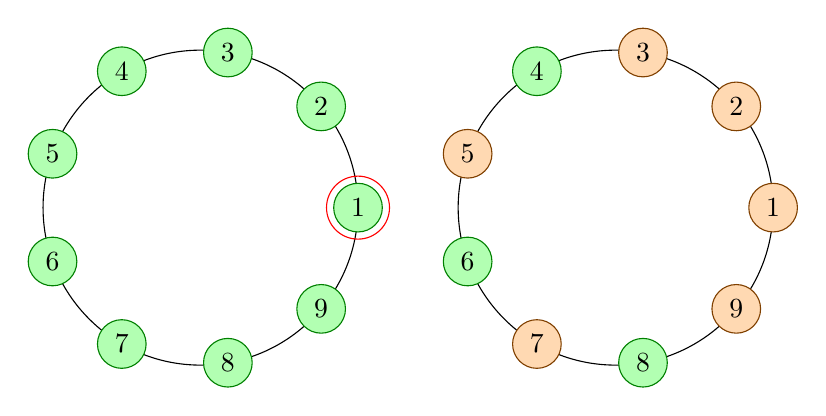
\begin{tikzpicture}[scale=0.5]
		    \begin{scope}
		      %\draw[->, bend right=12] (v0) to (v40);
		      \draw (0, 0) circle(4);
		      \foreach \i/\j in {0/1, 40/2, 80/3,120/4,160/5,200/6,240/7,280/8,320/9} {
		        \node (v\i) at (\i:4) [circle,fill=green!30!white, draw=green!50!black] {\j};
		      }
		      \draw[color=red] (0:4) circle(0.8);     
		    \end{scope}
		    \begin{scope}[xshift=300]
		      \draw (0, 0) circle(4);
		      \foreach \i/\j in {0/1, 80/3,160/5,240/7,320/9, 40/2} {
		        \node (v\i) at (\i:4) [circle,fill=orange!30!white, draw=orange!50!black] {\j};
		      }
		      \foreach \i/\j in { 120/4, 200/6, 280/8} {
		        \node (v\i) at (\i:4) [circle,fill=green!30!white, draw=green!50!black] {\j};
		      }
		    \end{scope}
      \end{tikzpicture}
    \end{center}
    \vspace{0.3cm}

  \item
    У Винни-Пуха есть бесконечные запасы каждого из $k$ типов горшочков мёда.
    Каждый тип горшочков характеризуется целым числом --- сколько дней нужно Винни-Пуху, чтобы съесть весь мёд из одного такого горшка.
    Винни-Пух уже провёл серию экспериментов вида ``взять несколько горшочков мёда, записать день недели, когда эксперимент начался, есть
    мёд, пока тот не закончится, записать день недели, когда эксперимент закончился'' (в наборе может быть несколько горшочков одного типа, в неделе 7 дней).
    По понятным причинам Винни очень любит экспериментировать. А Кролик не любит мёд, но любит предсказывать будущее. Помогите Кролику
    определить, можно ли, зная результаты первых $k$ экспериментов и набор горшков и день начала для $(k + 1)$-го,
    предсказать день недели, когда $(k + 1)$-й эксперимент закончится.
    \begin{enumerate}
      \item Для каждого эксперимента Винни берёт произвольные наборы горшков. $\O(k^3)$
      \item Для каждого эксперимента Винни берёт горшки не более чем двух разных типов. $\O(k)$.
    \end{enumerate}

\end{enumerate}
